% Name: Centroid and medians
% Description: Each median joins a vertex to the midpoint of the opposite side, and the three meet at the centroid G, two thirds of the way along each.
% Tags: centroid, medians, midpoint, triangle centers

\usetikzlibrary{calc}

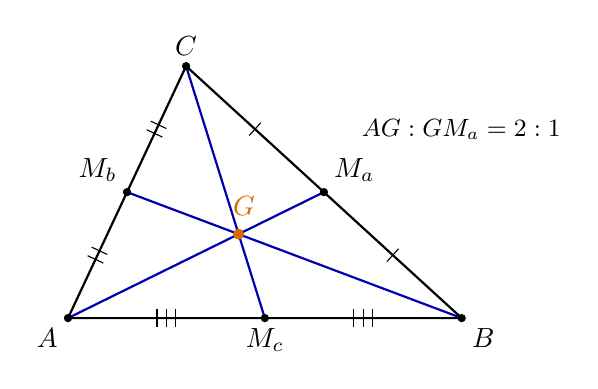
\begin{tikzpicture}[thick]
  \coordinate[label=below left:$A$] (A) at (0,0);
  \coordinate[label=below right:$B$] (B) at (5,0);
  \coordinate[label=above:$C$] (C) at (1.5,3.2);
  \coordinate[label=above right:$M_a$] (Ma) at ($(B)!0.5!(C)$);
  \coordinate[label=above left:$M_b$] (Mb) at ($(A)!0.5!(C)$);
  \coordinate[label=below:$M_c$] (Mc) at ($(A)!0.5!(B)$);
  \coordinate (G) at ($1/3*(A) + 1/3*(B) + 1/3*(C)$);
  \draw (A) -- (B) -- (C) -- cycle;
  \draw[blue!70!black] (A) -- (Ma) (B) -- (Mb) (C) -- (Mc);
  % One tick on each half of BC, two on CA, three on AB
  \foreach \p/\q/\n in {B/Ma/1, Ma/C/1, A/Mb/2, Mb/C/2, A/Mc/3, Mc/B/3}
    \foreach \k in {1,...,\n}
      \draw[thin] ($(\p)!0.5!(\q)!{(\k-(\n+1)/2)*1.2mm}!(\q)$) ++(0,0) coordinate (T) ($(T)!1.1mm!90:(\q)$) -- ($(T)!1.1mm!-90:(\q)$);
  \fill[orange!85!black] (G) circle (2pt) node[above=3pt, xshift=2pt] {$G$};
  \foreach \p in {A, B, C, Ma, Mb, Mc} \fill (\p) circle (1.5pt);
  \node[font=\small, anchor=west] at (3.6,2.4) {$AG : GM_a = 2 : 1$};
\end{tikzpicture}
